% A LaTeX (non-official) template for ISAE projects reports
% Copyright (C) 2014 Damien Roque
% Version: 0.2
% Author: Damien Roque <damien.roque_AT_isae.fr>

\documentclass[a4paper,11pt]{article}
\usepackage{polski}
\usepackage[utf8]{inputenc}
\usepackage{amsmath}
\usepackage{graphicx}
\usepackage{esvect}
\usepackage{caption}
\usepackage{indentfirst}
\usepackage{float}


\begin{document}
\begin{titlepage}
\begin{center}


{\large Nazwa kursu: Badania operacyjne w AIR}\\[0.5cm]

{\large Data odbytych zajęć: 25.10.2016}\\[0.5cm]

% Title
\rule{\linewidth}{0.5mm} \\[0.4cm]
{ \huge \bfseries Sprawozdanie: Maksymalny przepływ w sieci \\[0.4cm] }
\rule{\linewidth}{0.5mm} \\[1.5cm]

% Author and supervisor
\noindent
\begin{minipage}{0.4\textwidth}
  \begin{flushleft} \large
    \emph{Autorzy :}\\
    Sławomir Żaba 209165,\\
    Mateusz Wojdyła 209410 \\
  \end{flushleft}
\end{minipage}%
\begin{minipage}{0.4\textwidth}
  \begin{flushright} \large
    \emph{Prowadzący kurs :} \\
    Dr inż. Mariusz Makuchowski \\
  \end{flushright}
\end{minipage}
\end{center}
\end{titlepage}
\section{Cel ćwiczenia}
    Zadaniem na drugie laboratorium było zaimplementowanie algorytmu rozwiązującego problem maksymalnego przepływu w sieci. W problemie tym musimy określić maksymalną wielkość przepływu ze źródła do ujścia sieci przy ograniczeniach przepustowości nałożonych na poszczególne kanały. \\
    Problem ten rozwiązuje algorytm Edmondsa – Karpa, który w tym zadaniu zastosowano. jest jedną z realizacji metody Forda-Fulkersona rozwiązywania problemu maksymalnego przepływu w sieci przepływowej, z dodatkowym warunkiem: ścieżka powiększająca, którą szukamy w każdym kroku algorytmu, musi być najkrótsza, czyli zawierać minimalną możliwą ilość krawędzi. Taką ścieżkę znajduje się uruchamiając algorytm przeszukiwania grafu wszerz w sieci rezydualnej.
    
\section{Opis dodatkowych algorytmów}
    \textbf{Algorytm Forda-Fulkersona} stosowana do znajdowania maksymalnego przepływu w sieci przepływowej. Stanowi podstawę wielu algorytmów, między innymi algorytmu Edmondsa-Karpa czy algorytmu Dynica. Opiera się on na idei sieci rezydualnych oraz ścieżek. Zasadę jej działania można streścić w następujący sposób: Należy zwiększać przepływ wzdłuż dowolnej ścieżki ze źródła do ujścia, dopóki jest to możliwe \\
    
    \textbf{Algorytm przeszukiwania grafu wszerz} - jeden z najprostszych algorytmów przeszukiwania grafu. Przechodzenie grafu rozpoczyna się od zadanego wierzchołka s i polega na odwiedzeniu wszystkich osiągalnych z niego wierzchołków. Wynikiem działania algorytmu jest drzewo przeszukiwania wszerz o korzeniu w s, zawierające wszystkie wierzchołki osiągalne z s. Do każdego z tych wierzchołków prowadzi dokładnie jedna ścieżka z s, która jest jednocześnie najkrótszą ścieżką w grafie wejściowym. Algorytm działa prawidłowo zarówno dla grafów skierowanych jak i nieskierowanych.
\newpage
\section{Wyniki pomiarów}
    Program przetestowano na następujących grafach:
    \begin{figure}[H]
        \centering
            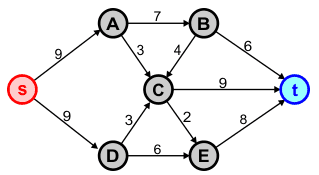
\includegraphics[width=0.4\textwidth]{in1}
            \caption{Graf pierwszy}
    \end{figure}
    \begin{figure}[H]
        \centering
            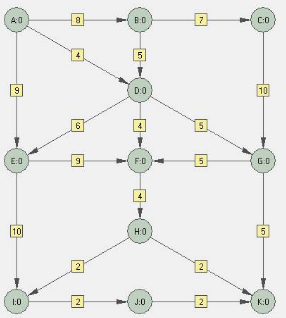
\includegraphics[width=0.4\textwidth]{in2}
            \caption{Graf drugi}
    \end{figure}
    \begin{figure}[H]
        \centering
            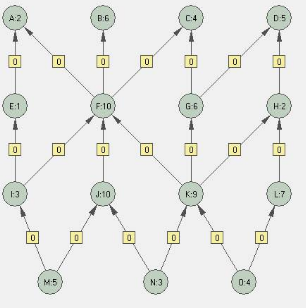
\includegraphics[width=0.4\textwidth]{in3}
            \caption{Graf trzeci}
    \end{figure}
    \newpage
    Dla powyższych grafów otrzymaliśmy następujące wyniki: \\[0.3cm]
    \begin{tabular}{c|c|c}
        Nazwa grafu & Maksymalny przepływ & czas wykonania programu [ms] \\ \hline
        graf pierwszy & 18 & 0.039 \\
        graf drugi & 9 & 0.17 \\
        graf trzeci & 0 & 0.026 \\ \hline
    \end{tabular}
    \captionof{table}{Wyniki programu dla poszczególnych grafów}
    \vspace{0.3cm}
    Program napisany przez nas oprócz podania maksymalnego przepływu oraz czasu wykonywania, wypisuje również kanały przez które przepływ nie płynie i są zbędne, a także pełną sieć rezydualną. Poniżej przedstawiono przykładowe wyjście programu dla grafu pierwszego: \\ \\
    \textbf{Maksymalny przeplyw:} 18 \\
    \textbf{Przeplywy:} \\
    1 $->$ 0 : 9 z mozliwych: 9 \\
    1 $->$ 2 : 1 z mozliwych: 7 \\
    2 $->$ 1 : 6 z mozliwych: 6 \\
    3 $->$ 1 : 3 z mozliwych: 3 \\
    3 $->$ 4 : 3 z mozliwych: 3 \\
    3 $->$ 6 : 3 z mozliwych: 9 \\ 
    4 $->$ 0 : 9 z mozliwych: 9 \\
    5 $->$ 4 : 6 z mozliwych: 6 \\
    5 $->$ 6 : 2 z mozliwych: 8 \\
    6 $->$ 2 : 6 z mozliwych: 6 \\
    6 $->$ 3 : 6 z mozliwych: 6 \\
    6 $->$ 5 : 6 z mozliwych: 6 \\ \\
    
    \textbf{kanaly niewykorzystane:} \\
    2 $->$ 3 : 4 z mozliwych: 4 \\
    3 $->$ 5 : 2 z mozliwych: 2 \\ \\
    
    \textbf{czas wykonania:} 0.039ms
\section{Wnioski}
TO DO!
\end{document}
